\documentclass[11pt]{article}

\usepackage[letterpaper,margin=1in]{geometry}
\usepackage{times}
\usepackage{amsmath}
\usepackage{url}
\urlstyle{rm}
\usepackage{graphicx}
\usepackage{xspace}
\usepackage{authblk}
\usepackage{cite}

%\documentclass[times, twoside, watermark]{zHenriquesLab-StyleBioRxiv}
%\usepackage{booktabs}
%\usepackage{lineno}
\usepackage{xr}

% To handle cross-referencing between documents
\makeatletter
\newcommand*{\addFileDependency}[1]{% argument=file name and extension
  \typeout{(#1)}
  \@addtofilelist{#1}
  \IfFileExists{#1}{}{\typeout{No file #1.}}
}
\makeatother

\newcommand*{\myexternaldocument}[1]{%
    \externaldocument{#1}%
    \addFileDependency{#1.tex}%
    \addFileDependency{#1.aux}%
}

\myexternaldocument{extra_insight_supplement}

\renewcommand{\baselinestretch}{1.5} % line spacing
\setlength{\parskip}{1em} % paragraph spacings
\renewcommand\Authfont{\fontsize{10}{10}\selectfont} % author font size
\renewcommand\Affilfont{\fontsize{9}{9}\selectfont} % affil font size
%\renewcommand{\abstractname}{\vspace{-\baselineskip}} % remove abstract
%\usepackage{caption}
%\captionsetup{font={large,stretch=1}} % legend font size and spacing

\newcommand{\mathbb}[1]{\boldsymbol{\mathbf{#1}}}

% add this for ref animation
\usepackage{prettyref}
\newrefformat{Sfig}{fig. S\ref{#1}}
\newrefformat{fig}{fig. \ref{#1}}

% command to indicate text WIP
\newcommand{\placeholder}{\textbf{(placeholder)}}

\linespread{1.15}
\title{Global characterization of mutations of large \\
  selective effect in the human genome}
%\title{Non-coding ultra-strong selection in the human genome varies by regulatory role and phylogenetic conservation}
%\leadauthor{Dukler}
%\shorttitle{ExtRaINSIGHT}
\author[1]{Noah Dukler}
\author[1]{Mehreen R. Mughal}
\author[2]{Yi-Fei Huang}
\author[1]{Adam Siepel}

\linespread{1.15}
\affil[1]{Simons Center for Quantitative Biology, Cold Spring Harbor Laboratory, Cold Spring Harbor, NY}
\affil[2]{Department of Biology and Huck Institutes of the Life Sciences, University Park, PA}
\date{}

\begin{document}

\maketitle

%\begin{keywords}
%Selection | Population Genetics | Human Genetics
%\end{keywords}

\begin{abstract}
% Understanding the impact of new mutations on fitness is a longstanding problem in evolutionary genomics.  
  Recently, genome sequencing of tens of thousands of human individuals has enabled the measurement of large selective effects for mutations to protein-coding genes, corresponding to fitness losses of as much as 1--30\%.  Here we describe a new method, called ExtRaINSIGHT, for measuring similar selective effects in noncoding as well as in coding regions of the human genome.  ExtRaINSIGHT estimates the prevalance of strong purifying selection ($\lambda_s$) as the fractional depletion for rare variants (minor allele frequency $<0.1$\%) in a target set of genomic sites relative to matched sites that are putatively neutrally evolving, in a manner that controls for local variation and neighbor-dependence in mutation rate.
%  
We show using simulations that, above an appropriate threshold, the score $\lambda_s$ is closely related to the average site-specific selection coefficient against heterozygous mutations, as predicted at mutation-selection balance.
 %
 Applying ExtRaINSIGHT to 71,702 whole genome sequences from gnomAD v3,
%check number  
we find that $\lambda_s$ is generally concordant with previous results at features in and around protein-coding genes.  Splice sites display the highest levels in the genome of strong selection against new mutations ($\lambda_s=0.48$), with somewhat lower levels for nonsense mutations ($\lambda_s=0.23$) and mutations to untranslated regions ($\lambda_s< 0.03$).
 % Neuronal genes (and...?) are enriched for strong selection, whereas.....
Among annotated noncoding elements, 
mature microRNA seed regions exhibit the strongest purifying selection ($\lambda_s =  0.38$),
  whereas lincRNAs and other noncoding RNAs display considerably reduced evidence of strong selection ($\lambda_s < 0.01$).
 Ultra-conserved elements ($\lambda_s = 0.09$) and human accelerated elements ($\lambda_s = 0.04$) display only moderate evidence of strong selection, suggesting that  
  their extreme conservation over millions of years of evolution results primarily from weaker purifying selection distributed evenly across many nucleotides.
  % something about genetic load result -- have to update this
  Our analysis suggests.....[genetic load result]
Our analysis also reveals highly atypical mutation rates in the upstream regions of genes, making it difficult to obtain accurate measurements there.  Overall, these methods shed new light on the genome-wide distribution of fitness effects for new mutations by combining deep new sequencing data sets and classical theory from population genetics.

  %The rapid expansion of human population whole genome sequencing data has resulted in an extensive catalog of rare variation. We use this rare variation as a proxy for \textit{de novo} mutation and construct a context-dependent model to predict rates of mutation genome-wide. The model also implicitly corrects for local factors, like replication timing, which are known to influence mutation rate using variation in the rates of rare variants in proximal neutral regions. We then compare the predicted versus observed rates of rare variation for groups of elements and discover those with fewer rare variants than expected. This depletion in rare variation is caused by strong purifying selection on the collection of elements where any mutation results in a large fitness penalty. We contrast this measure of strong selection with a measure of generalized selection to estimate the relative fraction of sites under weak and strong selection across both coding and non-coding regions. Consistent with previous work we find that the genes associated with neuronal function are most strongly depleted for rare variation while those associated with reproduction enriched relative the genomic background. By applying our method to non-coding regions we find that splice sites are the most strongly conserved followed by conserved microRNAs which show less variation than non-degenerate coding regions. Surprisingly we observe relatively little ultra-strong selection in humans in non-coding regions that show strict and deep phylogenetic conservation suggesting that they may be maintained by either pervasive weak selection or are tolerant to heterozygous mutation.  We also observed excess rare variation across a variety of elements that are inherently tied to biochemical function indicating that improvements in separating selection and mutation will require new approaches. Finally we have made the method we developed for this analysis, ExtRaINSIGHT, available as a web-tool for others to use.

\end{abstract}

\section*{Introduction}

Like a gambler, an evolving species has to pay for the chance to win.   In the game of evolution, this payment takes the form of deleterious mutations.  As in most games of chance, the majority of ``draws'' result in a loss (decrease in fitness) with an occasional pay-off (adaptive mutation).  In Haldane's words, loss of fitness owing to deleterious mutation is the ``price paid by a species for its capacity for further evolution'' \cite{HALD37}.

Understanding the impact of new mutations on fitness has has been a major focus of evolutionary genetics for nearly a century \cite{FISH22,HALD27,HALD37}. Together with genetic drift and natural selection, mutation is one of three primary evolutionary forces and the only force that can generate new genetic variation.  In this way, mutation is the fuel that enables natural selection to do its work.  Because fitness effects occur on a continuum, the general problem is to characterize the distribution of fitness effects (DFE) of new mutations.  Estimating the DFE is central in addressing a wide variety of fundamental problems in evolutionary genetics, including understanding the genetic architecture of complex traits, the emergence of recombination and sex, the behavior of populations maintained at small population sizes (as with domesticated animals and plants), and the effects of mutational load \cite{EYREKEIG07}.

%[something about human disease]
% another citation for load?  or is this one ok?

At the same time, characterizing the DFE is notoriously difficult.  Naturally occurring mutations are rare, they are often difficult to detect, and their fitness effects are hard to measure, especially when subtle (as is typical).  In model organisms, a variety of innovative experimental techniques have been developed to enable measurement the DFE, including mutagenesis and mutation accumulation experiments, although these methods tend to produce estimates with large confidence intervals, are useful only for mutations of relatively large effect, and may not otherwise be representative of spontaneously occurring mutations.  Moreover, these methods cannot be applied to humans, or, indeed, to any type of organism that cannot be experimentally manipulated and monitored in relatively large numbers.

For these reasons, recent efforts to characterize the DFE have focused on the use of statistical modeling, population genetic theory, and large-scale DNA sequence data.  In humans, these statistical methods are the only practical means for characterizing the DFE, and in all organisms, they have the advantage of providing access to a collection of naturally occurring mutations of both small and large effect.
Over the past two decades, various versions of this strategy have been devised, including ones that make use of patterns of
divergence across species \cite{KIMU77,KONDCROW93,NIELYANG03,EYREKEIG99},  
combinations of patterns of polymorphism and divergence \cite{MCDOKREI91,SAWYHART92,BUSTETAL02,ARBIETAL13},
the full site-frequency spectrum in human populations \cite{EYREETAL06,BOYKETAL08,HUANSIEP19},
and rates of protein-truncating variants at dominant or X-linked disease-associated genes \cite{KOND03}.   % maybe don't keep this one?

Nevertheless, these strategies have some important limitations.  In particular, patterns of variation are strongly influenced by demographic history, especially by population bottlenecks, expansions, and substructure, so that careful demographic modeling is required to isolate the effects of selection.  In addition, the population panels that are typically available---consisting of hundreds to a few thousand individuals---are informative about only a relatively narrow slice of the DFE.  For example, in humans strong purifying selection (such that $s$ is larger than $\sim$1\%) will tend to hold variants to such low frequencies in the population that they will not be reliably detectable in these panels, whereas weak purifying selection (such that $s$ is on the order of $10^{-4}$ or less) will be indistinguishable from random genetic drift.  Thus, only in approximately the range $10^{-4} < s < 10^{-2}$  is there any hope of accurately measuring the strength of purifying selection.

In recent years, several large consortium projects have released public genome sequence data (either at the exome or the whole-genome level) for several thousand human individuals \cite{FUETAL13,1KGCONS15,LEKETAL16,KARCETAL20}.  The largest of these data sets now span many tens of thousands \cite{LEKETAL16,KARCETAL20}, allowing quite rare variants (with frequencies of $<10^{-3}$) to be identified with reasonable confidence.  With this capability in mind, a number of statistical methods have been developed to measure high levels of purifying selection against loss-of-function mutations for protein-coding genes, by comparing the frequencies of predicted loss-of-function (pLoF) variants to their mutation-rate-based expectation \cite{PETRETAL13,LEKETAL16,KARCETAL20,CASSETAL17,HAVRETAL19}.
Perhaps the most widely used of these are the ``probability of being loss-of-function intolerant'' (pLI) measure, and its successor, the loss-of-function observed/expected upper bound fraction (LOEUF) measure, both of which have been shown to reliably distinguish null (unconstrained), autosomal recessive, and haploinsufficient genes and to be associated with a number of other measures of molecular function and disease association \cite{LEKETAL16,KARCETAL20}.

While these measures are correlated with dominance effects, the frequency of rare pLoF variants is strictly informative only about the strength of selection against hetereozygous mutations, here denoted $s_{\text{het}}$~\cite{FULLETAL19}.  When selection is strong and near-complete recessivity can be excluded, mutation-selection balance is expected to hold with an equilibrium frequency for a rare variant of $q \approx \frac{\mu}{s_{\text{het}}}$, where $\mu$ is the deleterious mutation rate \cite{HALD37,FULLETAL19}.  Indeed, Cassa et al.\ \cite{CASSETAL17} and Weghorn et al.\ \cite{WEGHETAL19} have shown with extensive simulations that this relationship holds quite well for pLoF variants in the ExAC exome data \cite{LEKETAL16} down to $s_{\text{het}} \approx 0.01$.  Their approach allows for direct estimation of selection coefficients as large as $s_{\text{het}} =0.3$ or more, and they identified thousands of human genes with estimated $s_{\text{het}} >0.1$ for pLoF.
Importantly,  estimation of $s_{\text{het}}$ based on mutation-selection balance
is independent of demography because, in this regime, mutant alleles persist in the population for at most a few generations and genetic drift makes a negligible contribution to their allele frequencies.
Therefore, in addition to permitting estimation of larger selection coefficients than other statistical methods, this approach requires no demographic modeling.


%Exome Aggregation Consortium (ExAC)

In this paper,
we develop method noncoding regions
similar to methods for coding regions -- mutation rates

We derive the method.....
fractional decrease in rare variants

however, for sufficiently strong selection
can be interpreted as an estimator for shet
based on mutation-selection balance similar to Cassa et al



apply to gnomAD

To date, the largest publicly available whole-genome sequence data set is the Genome Aggregation Database (gnomAD), which, at first publication, consisted of 15,708 individuals \cite{KARCETAL20}, 
and in v3.1.1 has expanded to 76,156 individuals (https://gnomad.broadinstitute.org/).

characterize the presence of very strong selection
(``ultra-strong selection'')



%%%%




%Recent efforts at cataloging human genetic variation such as the 1000 Genomes Project (cite) and the Simons Genomic Diversity Panel (cite) resulted in extensive annotation of common genetic variants. These variants have illuminated a complex history of migration and admixture, both within modern humans and in their interactions with archaic hominins. Inferring demographic histories and distributions of selective effects have been the two most ubiquitous goals in population genetics, and while common variants have been essential for the former, they have had limited power for the latter. Usually, the presence of purifying selection is detected by a depletion of genetic variation within a region, however common variants are unable to differentiate between sites under weak or strong selection as both will prevent a variant from rising to high frequency in a population (cite). Recent projects with the aim of massively expanding the number of sequenced whole genomes such as (...) have provided an expansive view of rare human variation not previously available. Unlike common variants, rare variants are not efficient for inferring broad population structure but they can be used to differentiate between weak and strong purifying selection (cite).

%Several approaches have been developed that utilize rare variation data to find collections of sites that show extreme depletion for such variants (cite UNEECON, petrovski 2013, etc. ). One of the most widely used of these is pLI (cite) which uses loss-of-function (LoF) variants to label proteins as being haplo-insufficient (intolerant to single copy loss) or haplosufficent. Rare variation is associated with haplosufficiency because rare variants are almost always heterozygous, thus a depletion of a rare variant is usually observed as intolerance to even a single copy of that variant. Other approaches such as CCR (cite - Havrilla 2019) have improved upon the resolution of pLI, looking for signals of ultra-strong constraint at the sub-domain level. A caveat that was raised in recent commentary has pointed is that approaches like pLI ``reflect the strength of selection acting on heterozygotes and not dominance or haploinsufficiency''(cite - Fuller 2019). Thus signals of constraint from rare variants are actually the product of the dominance coefficient $d$ and the selection coefficient $s$.

%While these methods are all quite powerful, because they exploit the DNA to protein sequence mapping, they apply solely to coding regions. This excludes $\sim 99\%$ of the genome from analysis, excluding a number of interesting regions (including ultra-conserved non-coding elements) from analysis. We developed ExtRaINSIGHT to overcome this limitation, at the cost of some nuance in protein coding regions, by creating a globally applicable model for the probability of observing rare variants in neutrally evolving regions. This work probes the role of strong selection in shaping both coding and non-coding elements stratified by function.

\section*{Results}

\subsection*{Overview of ExtRaINSIGHT}

The conceptual basis of ExtRaINSIGHT is straightforward: as noted, the method attempts to measure the fractional reduction in the presence of rare variants in a target set of sites relative to nearby sites that are putatively free from (direct) effects of natural selection.  

In this way, the method is analogous to classical divergence-based approaches \cite{}
%such as the measurement of Ka/Ks (or dn/ds) from alignments of divergent protein-coding sequences or of XXXX (Crow),
as well as to newer methods that compare target sets of noncoding elements with suitable background sequences in terms of divergence (CITE phastCons, phyloP, GERP), polymorphism (CITE Ekta, Huang, others), or polymorphism and divergence (CITE INSIGHT, LASSIE),

but the focus on rare variants (here, variants with minor allele frequencies of $< 0.1$\%) enables the method to shed light on mutations of large selective effect.

The main challenge in this approach stems from the high sensitivity of relative rates of rare variants to variation in mutation rate.  To address this problem, we follow Lek et al...... (others?)
and make use of a 
hexamer model.....

In addition, following our earlier work (cite), we use a local control for mutation rate
by identifying collections of sites likely to be neutrally evolving (by liberally excluding annotated functional elements and other sites likely to be under selection; see Methods)
and including in the model a scale factor for mutation rate at each target sites based on nearby ``neutral'' sites

With this strategy,
we are able to predict with high accuracy the probability that a rare variant will occur at each site
denoted $P_i$
%[show validation experiment]

%%%

In the absence of natural selection, we assume a  binomial sampling model for the presence (probability $P_i$) or absence (probably $1-P_i$) of a rare variant at each site $i$, excluding sites at which common variants occur (similar to.... GNOMAD).
where $P_i$ is determined by the local sequence context and local rate constant.  Assuming independence, the probability of a collection of nucleotide sites is given by,
\begin{equation}
P(\mathbb{Y}; \mathbb{P}) = \prod_i P_i^{Y_i}(1-P_i)^{1-Y_i}
\end{equation}
\noindent where $Y_i$ is an indicator variable for the presence of a rare variant at position $i$ in the sample.

We then assume that natural selection has the effect of imposing a fractional reduction on the rate at which rare variants occur.  that is,....
\begin{equation}
  P(\mathbb{Y}; \lambda_s, \mathbb{P}) = \prod_i \left[(1-\lambda_s) P_i\right]^{Y_i}\left[1- (1-\lambda_s) P_i\right]^{1-Y_i}
\end{equation}
\noindent where $\lambda_s$ is the scale factor capturing a depletion of rare genetic variation.  Assuming the $P_i$ values are pre-estimated, a maximum-likelihood estimate (MLE) of $\lambda_s$ can be obtained in closed form (see Methods).

When $\lambda_s$ falls between 0 and 1 it can be interpreted as a measure of the prevalence of strong purifying selection,
i.e., selection sufficiently strong that mutations are either lethal and never occur or tend to be eliminated within a few generations and are never allowed to drift to appreciable frequency
This value can be thought of as fraction of sites intolerant to heterozygous mutants, although in practice, some sites may be more, and some sites less, intolerant

Notice, however, that $\lambda_s$ can also take values $<0$
suggesting that rare variants are occurring at a higher-than-expected rate in a target set of sites
As we discuss below, we do observe a systematic tendency for lambda to take negative values in particular classes of sites, likely reflecting the difficulty of precisely specifying the mutational model at these sites.
Across most of the genome, however, estimates of lambda fall between 0 and 1 and show general qualitative agreement with what is expected for various types of functional elements.

%---
%(now switch to popgen theory)
Notably, in the case of strong selection against heterozygotes and mutation-selection balance (as studied by [refs]),
a relatively simple nonlinear relationship can be established between $\lambda_s$ and the (average) site-specific selection coefficient against heterozygous mutations, $s_h$:    ......     [maybe leave constants vague]     [show in a figure]
where $c$ is a constant that depends on the relative values of the per-generation mutation rate and the rate of presence of rare variants, $P_i$ (see Methods).
% just say ratio

Following the example of Weghorn et al., we carried out a series of simulations 
under various values of $s_h$, 
a plausible demographic model (?)
and found that this approximate relationship was fairly accurate down to about $s_h = 10^{-2}$ (check)
The observation parallels and is similar to the one reported by Weghorn et al. but.... [differences]
In addition, we  found that the estimator was reasonably robust to variation across sites in mutation rate and in $s_h$ (Suppl Figs)   [other stuff], serving as a good indicator of the average $s_h$ at the target set of sites in such cases
Thus, for values of $\lambda_s$ larger than about 0.15 (CHECK), we can obtain a good estimate of the corresponding average sitewise selection coefficient.
%[indicate on the plot the approximate threshold of interest]

\subsection*{ExtRaINSIGHT is consistent with other measures of strong coding constraint}
As a validation for ExtRaINSIGHT we compared it with another method for detecting genes that were intolerant to heterozygous loss of function (LoF) variants, pLI. Genes were classified as rare variant tolerant (pLI $\leq 0.1$) or intolerant (pLI $\geq 0.9$). ExtRaINSIGHT found similar results to pLI using all CDS sites, with a larger fraction of sites being intolerant of heterozygous variants in genes that were classified as rare variant intolerant by pLI.  (As a secondary validation do we want to estimate per gene extraINSIGHT scores and show they similar, but probably slightly worse than pLI at prioritizing known recessive disease genes?) 

We then sought to estimate the relative fraction of sites under strong vs. weak selection by taking the ratio of $\lambda_s$ and $\rho$, a measure of the combined fraction of weak and strong selection presented in INSIGHT (cite). This ratio serves two purposes (1) de-convolving the relative contributions of weak and strong selection to the observed pattern of polymorphism and (2) controlling for the fraction of sites under purifying selection, allowing for more rigorous comparisons across annotations of varying quality. To have a baseline against which to compare the relative roles of weak and strong selection we estimate $\rho$ and $\lambda_s$ for coding and non-coding regions on a random subset of fifteen million sites for each. Using INSIGHT2 we find estimates of generalized purifying selection ( $\rho$ ) of $0.62$ for coding regions and $0.07$ consistent with previous findings. Applying ExtRaINSIGHT, we obtained estimates of $0.145$ and $0.008$ for the fraction of sites under ultra-strong selection for coding and non-coding sites, respectively. By taking the ratio $\frac{\lambda_s}{\rho}$, we find that $23.3\%$ of sites under purifying selection are under ultra-strong selection. In contrast the same calculation for non-coding elements results in an estimate of only $11.5\%$. Thus we find that strong selection is roughly twice as prevalent in coding elements as non-coding elements.

With this genome-wide baseline in hand we do the same calculation for the two categories of pLI genes previously described. Not only do genes high pLI scores show larger fraction of sites under purifying selection than those with low scores ($\sim 0.76$ vs. $\sim 0.6$), sites that are under purifying selection are roughly two and half times as likely to be under ultra-strong selection. This is consistent with the expectation organismal fitness is less impacted by single copy mutations in genes with low pLI, even those in functionally important sites, than those with high pLI scores.

\subsection*{Excess strong selection in neuronal genes}

Previous works has shown that the strength of selection on coding sequence varies between different classes of genes. We sought to investigate this with ExtRaINSIGHT by subdividing genes into distinct functional groups using top-level Reactome annotations and estimating the amount of ultra-strong selection in each class. Gene associated with neuronal system showed the highest relative abundance of strong selection in line with previous work studying autism showing that strong selection is prevalent in neuronal genes (cite pLI, ExAC?)(\prettyref{fig:reactome}). Autophagy was the next most enriched category of genes, likely because of the documented role of autophagy genes in neurodegenerative disorders (Stamatoku et al. 2020). Other categories that showed relatively large fractions of sites under ultra-strong selection include muscle contraction, DNA replication genes, and metabolism of RNA. Metabolism of RNA includes the genes responsible for splicing, so it is perhaps not surprising to see them here as splice sites themselves are particularly intolerant to mutation (cite Zhang 2018). Surprisingly, given that they are the canonical example for dosage sensitive genes (cite), genes annotated as being involved in gene expression (largely TFs) were not among those most enriched for strong selection. At the other extreme genes associated with reproduction showed the smallest role for strong selection as has been previously reported (cite). Unsurprisingly, metabolic genes, the canonical example for dosage insensitive genes, were also near the bottom of the list.

Where possible we sought to confirm these results using tissue specific gene expression as a source for orthogonal annotations. Genes were annotated as being specific to a given tissue using the ZZZ metric (cite) computed from GTEx data. All the genes most enriched for strong selection were tissue specific to various regions of the brain (\prettyref{Sfig:tissue_specific_scores}) supporting our previously seen enrichment for strong selection in nervous system genes. For reproductive genes the evidence is more mixed with neither ovaries nor testis coming out at the bottom of the list. (Not sure how to wrap this up)

\subsection*{Conserved microRNAs are strongly constrained}
While ExtRaINSIGHT can be applied to coding regions it distinguishes itself from previous work by being equally applicable to non-coding regions. However, one of the major challenges of studying the relative role of selection between types of non-coding sequence is the varying imprecision of most non-coding annotations. Thus, to investigate the role of ultra-strong in non-coding regions we chose core splice sites and microRNAs because of their characterized biochemical function and contrasted them with 1D coding sequence. Splice sites were under incredibly strong selection with $\sim45\%$ of sites being depleted for rare variation, twice the rate seen in 1D CDS. Both seed and non-seed regions of conserved microRNAs also showed $50\%-70\%$more strong selection than 1D CDS (\prettyref{fig:micro_rnas}A). This is likely due to the extreme dependence of microRNA function on a specific sequence and the highly pleiotropic effects of disrupting one (cite). In contrast, non-conserved microRNAs no evidence of strong selection.

\subsection*{Human accelerated and ultra-conserved regions show surprisingly similar amounts of ultra-strong selection}

Next we investigated two types of regions under dramatically different patterns of phylogenetic constraint. Ultra-conserved non-coding elements (UCNEs) are defined by extreme sequence conservation across broad swaths of phylogenetic time. In contrast human accelerated regions (HARs) show an excess of substitutions along the human lineage suggesting adaptation may be taking place (Pollard et al 2006). Naively we would expect that UCNEs would be extremely intolerant to mutation becasue of their deep conservation however that is not the case. Only $\sim 9\%$ of sites in UCNEs show evidence of ultra-strong purifying selection (\prettyref{fig:micro_rnas}B). There are several possible explanations for this: (1) UCNEs may largely be haplosufficent so heterzyogous variation is well tolerated, or (2) that UCNEs are under pervasive weak selection such that mutations are tolerated at the individual level but are sufficient to maintain near sequence identity across phylogenetic time. There is some evidence for this based on work in mice where deletions of UCNEs yielded viable and fertile individuals with no other obvious phenotypic defects (Ahituv et al. 2007). More recent work has provided examples of UCNEs that are haploinsufficient (Bhatia et al. 2013) or whose homozygous deletion leads to developmental defects (Dickel et al. 2018) but even in these cases individuals with these defects remained viable and fertile.

If UCNEs show unexpectedly little evidence of ultra-strong selection, HARs show a surprising amount despite also being almost entirely non-coding. Roughly $5\%$ of sites in HARs show ultra-strong selection, half that of UCNEs, despite being much more recently evolved. Several lines of evidence have implicated HARs in neuronal function with mutations in those regions being associated with cognitive disorders (Doan et al. 2016, Won et al 2019, Ryu et al 2018). This shows that just because function is recently evolved does not preclude it from being under ultra strong selection. 

\subsection*{Neutral mutation model mis-specification is observed due to hyper-local mutation rate variation is associated with TF binding}

ExtRaINSIGHT relies upon a neutral mutation model calibrated using putatively neutral regions to make inferences about whether a given set of sites is depleted or enriched for ultra-rare variants. In addition to sequence context the model adjusts for local mutation rate variation and excludes CpG sites to avoid issues arising from methylation dependent variation in mutation rate. This model is globally well calibrated across the whole spectrum of predicted mutation probabilities (supplemental figure 2). Despite this we observed that sets of sites that we would expect to be under selection were in fact inferred to have excesses of rare variation. This effect was most pronounced in the 1kb directly upstream of transcription start sites (TSS) and to a far lesser degree at 4D sites but not near the transcription termination sites (TTS)( \prettyref{fig:mutation_model_misspec} ). Given that it has been shown that proximal promoter region is under purifying selection (cite) we hypothesized that this is due to a local elevation of mutation rates directly upstream of TSS  (as has been shown in other species?(cite)). We further narrowed our focus to TFBS which have been previously observed to have elevated mutation rates (cite). When we looked within cannonical TFBS motifs we observed an excess of rare variants, even more so than in the X bp directly flankning the TFBS. This suggests that there are hyper-local determinants of mutation rate, in this case likely that the binding of TFs is itself mutagenic (cite). This poses a fundamental problem, all neutral models to date assume that mutation and function that exposes genomic sequence to selection can be decoupled for the purposes of estimating a neutral model, which does not hold here as TF binding is both inherently functional and mutagenic. Addressing this challenge will be critical not only for traditional evolutionary models but particularly for application in oncogenomics where excess mutations could give false signals of recurrent mutation leading to erroneous identification of cancer drivers (see discussion).

\section*{Methods}
\label{sec:materials:methods}
\subsection*{Creating a neutral mutation model}

To get a collection of rare variants to serve as a proxy for \textit{de novo} mutations, we filtered the gnomAD (v3) database (cite) keeping SNPs with an allele frequency of $\leq 0.001$. We removed all CpG sites to avoid the effects of methylation on CpG mutation and sites with an average sequencing coverage of $<20$. To calibrate the mutation model we needed a set of neutral regions for which we used the set we defined for the INSIGHT method(cite), lifting over to hg38 when necessary(cite liftOver). Finally, we constructed a set of features per allele at every site in the genome to be used in the mutation model. There were four features in the mutation model: frequency of each possible mutation given the 7-mer context in neutral regions, the log sequencing coverage, percent GC content in a 200bp window centered on the variant, and whether the SNP was in a CpG island based on \placeholder \textit{et al.}. We subsampled $1\%$ of mutations in these neutral regions and fit a logistic model to create a global model of \textit{de novo} mutation probabilities absent selection. To adjust for local factors that cause variation in the mutation rate (e.g. replication timing and recombination rate, cite), we tiled the genome into 50kb bins, then used the neutral variants per focal tile and flanking tiles with the mutation probability predicted from the global model as the only feature (plus an intercept) to produce a locally adjusted estimate of the mutation rate per variant. This procedure provides globally well calibrated estimates of mutation rates across all mutational frequencies (\ref{Sfig:mutation_model_calibration}).

\subsection*{Estimating the fraction of sites that are intolerant to heterozygous mutation}
Using our predictions to provide the rate of mutation ($P_i$) for any given site ($i$ under neutrality and assuming independence of sites we can detect deviations from the neutral mutation model by fitting this binomial likelihood model:

\begin{equation}
\mathcal{L}(\lambda ;\mathbb{Y},\mathbb{P}) = \prod_i ((1-\lambda_s) \cdot P_i)^{Y_i}(1- (1-\lambda_s) P_i)^{1-Y_i}
\end{equation}

\noindent where $\lambda_s$ is the scale factor capturing a depletion of rare genetic variation and $Y_i$ is an indicator variable for the presence of mutation $i$ in the sample. As noted previously, this observed depletion of rare variants is due to both dominance and selection, so $\lambda_s$ represents the fraction of sites where the combination of both factors is sufficiently deleterious for new mutations that even rare variants are not observed. As shorthand for this concept we will refer to $\lambda_s$ as measuring the fraction of sites under ultra-strong selection where larger values correspond to more sites under ultra-strong purifying selection. We then compute both a standard error using the curvature of the likelihood surface and a p-value using a likelihood ratio test for the following hypothesis set.

\begin{align}
H_0\text{(no selection) : } & \lambda_s = 0\\
H_1\text{(under selection) : } & \lambda_s \neq 0
\end{align}

Unlike other approaches (such as pLI) for detecting intolerance to rare variants, ExtRaINSIGHT is agnostic with regard to the functional impact of the rare variants in its database, and thus can be applied to both coding and non-coding regions.

\subsection*{Calculating the total number of sites under purifying selection}
By design, ExtRaINSIGHT will not detect weak purifying selection acting upon a region because it analyzes only rare variants. To contrast the relative abundances of weak and strong selection in a set of sites we turn to $\rho$, the metric for fraction of sites under combined weak and strong purifying selection introduced by the INSIGHT method. For this work we calculate $\rho$ using the updated version of INSIGHT, INSIGHT2 (cite). INSIGHT2 is only available on \textit{hg19} so only sites that have a 1-1 mapping between \textit{hg19} and \textit{hg38} are used in all analysis. Furthermore, all annotation sets with more than one million sites were sub-sampled to one million for computational efficiency unless otherwise stated.

\section*{Discussion}

\subsection*{Data Availability}

ExtRaINSIGHT and INSIGHT2 scores can be computed for a set of annotations using the ExtRaINSIGHT web portal at \url{http://compgen.cshl.edu/extrainsight}. All pipeline and analysis for this paper can be viewed on github at \placeholder.

\bibliographystyle{plos2015}
\bibliography{refs}

\begin{figure*}[t]
    \centering
    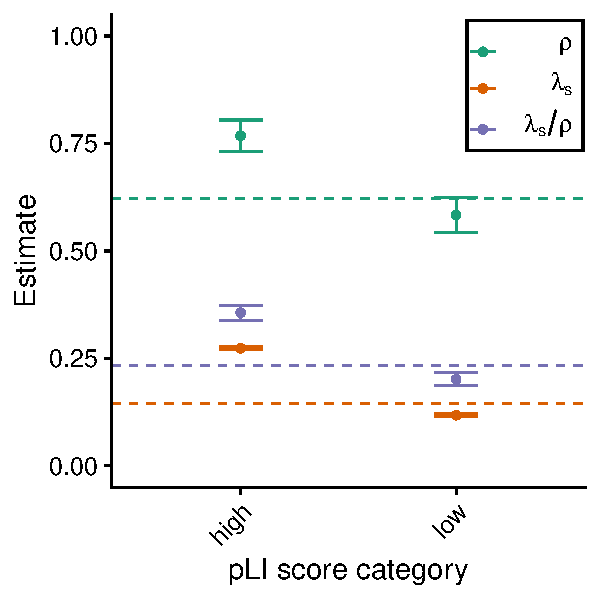
\includegraphics[width=0.5\linewidth]{figures/pLI_ratio.pdf}
    \caption{\textbf{Comparison of pLI and ExtRaINSIGHT scores in CDS}}
    \label{fig:pli}
\end{figure*}

\begin{table*}[t]
    \centering
	\begin{tabular}{@{}llll@{}}
%		\toprule
		Region     & $\rho$ & $\lambda_s$ & ratio  \\ %\midrule
		Coding     & 0.6219 & 0.1449     & 0.2330 \\
		Non-coding & 0.0664 & 0.0076     & 0.1150 \\ %\bottomrule
	\end{tabular}
	\caption{\textbf{Genome-wide estimates of generalized and strong selection.} Estimates were computed using  based on a random set 15 million sites per category. }
	\label{tab:genome_wide_scores}
\end{table*}

\begin{figure*}[t]
    \centering
    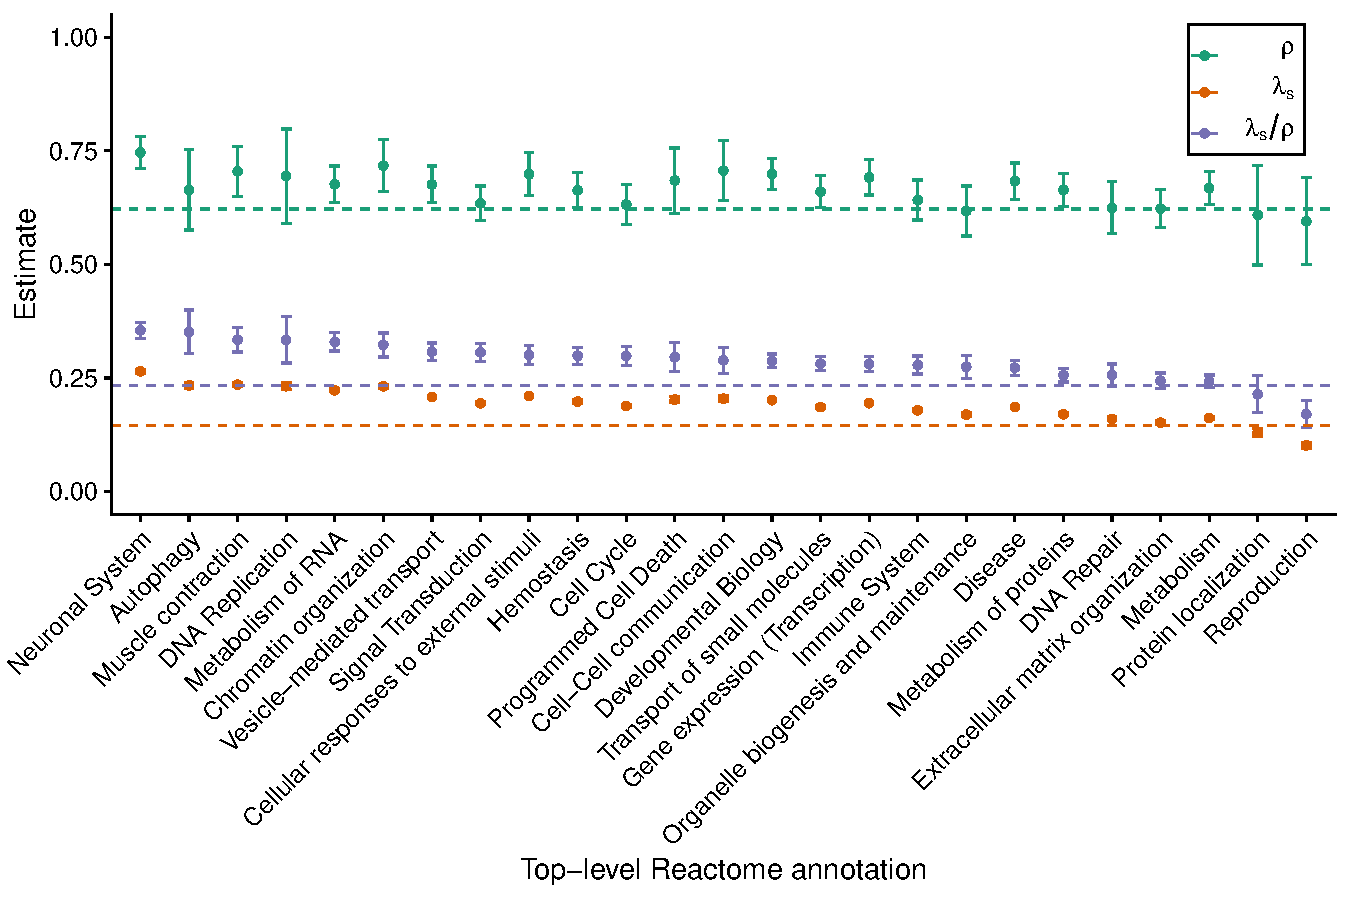
\includegraphics[width=\linewidth]{figures/reactome_cds_ratio.pdf}
    \caption{\textbf{\textbf{ExtRaINSIGHT scores in CDS stratified by biological pathway}}}
    \label{fig:reactome}
\end{figure*}

\begin{figure*}[t]
    \centering
    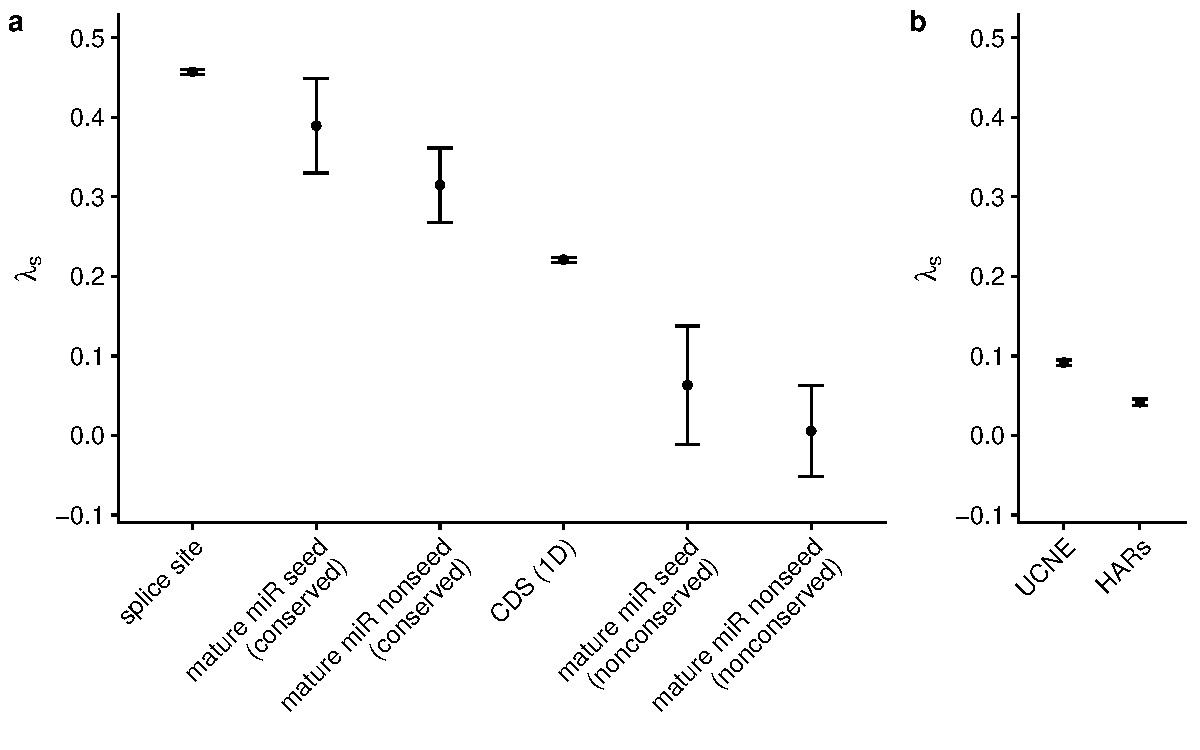
\includegraphics[width=\linewidth]{figures/microRNA_constraint.pdf}
    \caption{\textbf{\textbf{Heterozygous mutations in conserved microRNAs are under stronger selection than those in CDS}}}
    \label{fig:micro_rnas}
\end{figure*}

\begin{figure*}[t]
    \centering
    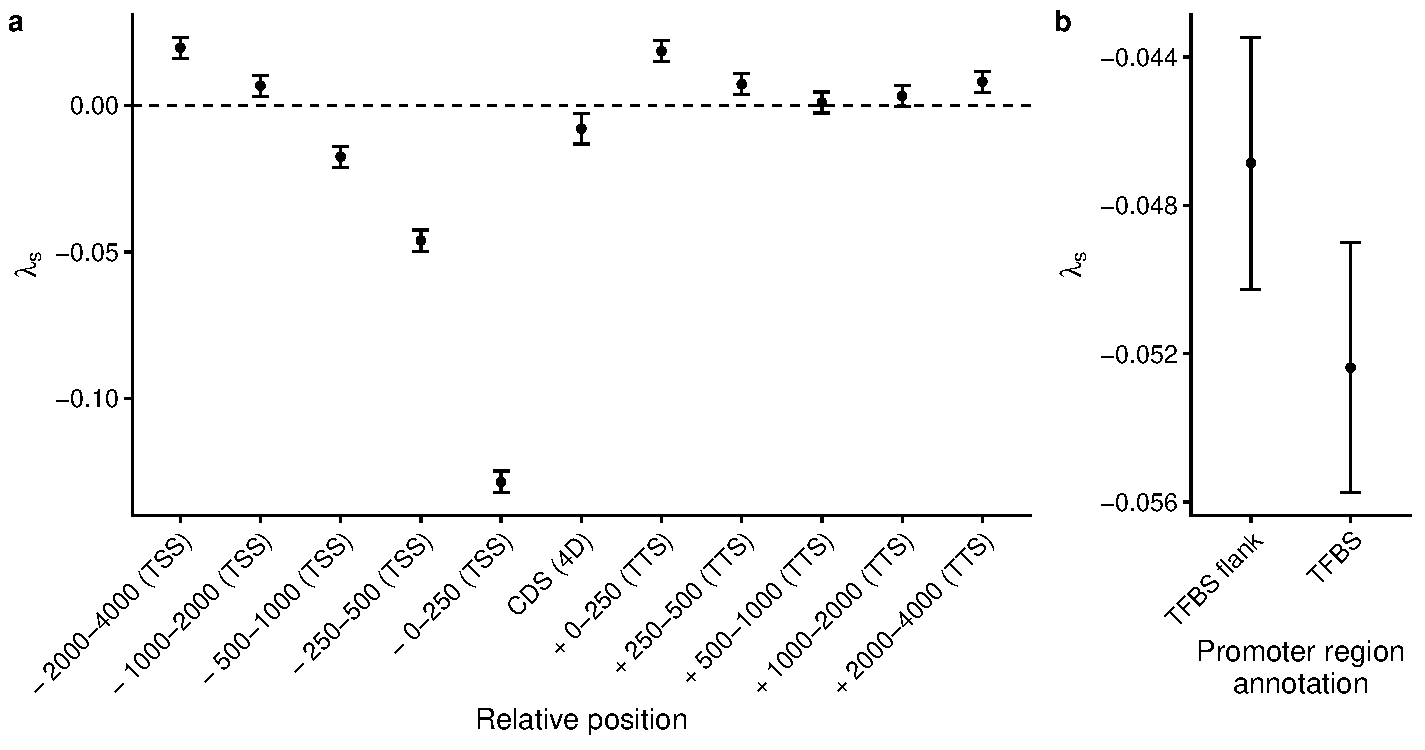
\includegraphics[width=\linewidth]{figures/excess_mutation_rate.pdf}
    \caption{\textbf{\textbf{TFBS show elevated mutation rates}}}
    \label{fig:mutation_model_misspec}
\end{figure*}



\end{document}